\section{System architecture}
\label{sec:sysarch}

This section describes the architecture of the interaction between the flight controller and the companion computer running the DroneVisionControl application outside of the simulation environment. It outlines the key components of the system along with their connections, discussing two possible configurations: offboard, where the companion computer acts as a ground station communicating wirelessly with the flight controller, and onboard, where the companion computer is physically connected with a cable to the flight controller so that they can fly together. The following sections explore the details of each configuration.

\subsection{Top-level components}

\begin{figure}
  \centering
  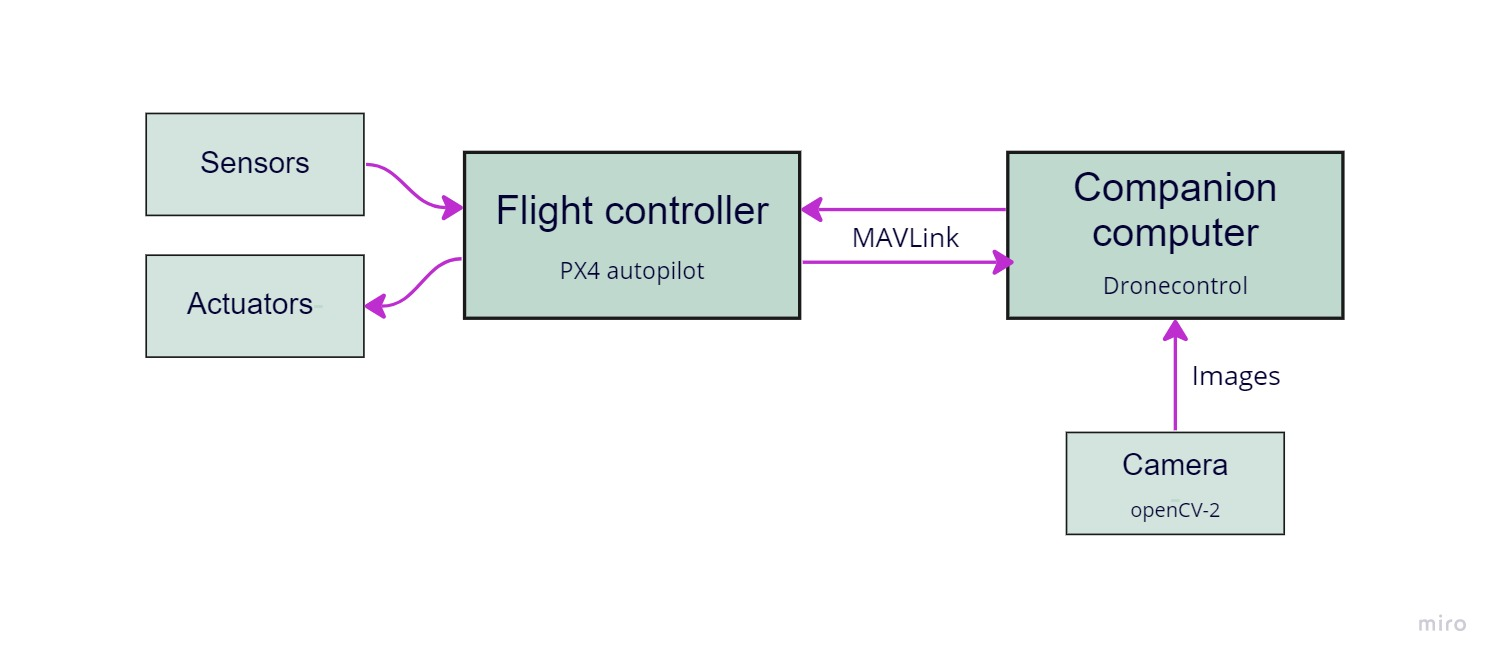
\includegraphics[width=0.9\textwidth,keepaspectratio]{img/sys-arch-diagram.jpg}
  \caption{Top-level diagram of the hardware/software interactions.}
  \label{fig:toplevel}
\end{figure}

The DroneVisionControl application aims to direct the movement of a UAV by analyzing images captured by a camera. Since the processing power needed to analyse the images exceeds the capabilities of the autopilot flight controller, an additional companion computer is necessary. This companion computer will control the camera and utilise machine learning algorithms to extract useful features from the images and convert them into movement directives for the vehicle.

Figure \ref{fig:toplevel} illustrates a top-level diagram depicting the key components of the system. The main elements include the flight controller, running the PX4 autopilot firmware, the companion computer hosting the developed application, and the camera responsible for image capture.  The camera connects to the companion computer using a USB cable plugged into any available port. The flight controller establishes the communication with the companion computer via the MAVLink protocol described in Section \ref{subsec:mavlink}, either through telemetry radios or a direct wire connection. The choice of connection type depends on the desired setup of the system.

In the simplest, offboard configuration, the companion computer can function as a ground station, directing the vehicle's movement from the ground while the flight controller remains onboard. This configuration is possible when the camera does not need to move with the vehicle. In this scenario, the only choice of communication is wireless, established utilizing a pair of telemetry radios. Section \ref{subsec:offboard} provides a comprehensive guide for this configuration.

Alternatively, when the camera needs to move with the vehicle to capture images from its perspective, the onboard configuration is used. In this scenario, the companion computer with its camera is placed onboard the vehicle alongside the flight controller. To communicate the two, a direct wired connection is the most suitable option, as it offers a faster and more reliable link than the telemetry radios. Details of this configuration are provided in Section \ref{subsec:onboard}.

\subsubsection{The flight controller}

The Pixhawk 4 board, designed for the PX4 autopilot, is integral to the project's autonomous flight control. This hardware depends on a set of sensors (gyroscopes, accelerometers, magnetometers, barometers) to determine the vehicle's state and actuators to translate controller outputs into physical movements. Additionally, a GPS or similar positioning system allows for automated flight modes and features like altitude stabilization.
In manual flight modes, a Radio Control (RC) system communicates control inputs from a remote unit to a vehicle-mounted receiver. Telemetry radios establish wireless MAVLink connections between ground control stations and PX4-powered vehicles, enabling dynamic parameter adjustments and mission modifications.
In actual UAVs, PX4 software runs on the dedicated Pixhawk hardware, whereas in simulated environments, all sensor and actuator components are emulated on the same computer.


\subsubsection{DroneVisionControl and the companion computer}

The DroneVisionControl application that runs on the companion computer utilizes the Python programming language\footnote{\url{https://www.python.org/}}. Python offers several advantages for projects of this nature, including its high-level, easy-to-use syntax, which results in a more concise code base compared to other languages. Other benefits include Python's versatility and support for object-oriented programming. Moreover, Python has a vast ecosystem of external libraries accessible through its official package manager called \texttt{pip}. This package index\footnote{\url{https://pypi.org/}} contains thousands of well-tested utilities, including many designed for machine learning and image processing. Additionally, Python versions of all the necessary libraries for interacting with PX4 via the MAVLink protocol, for object detection and tracking, and for simulation (MavSDK, OpenCV, AirSim, Mediapipe) are available. Being an interpreted language, Python can run seamlessly on any system with Python installed, eliminating the need to compile separate binaries to run in different operating systems.

The following sections will provide an in-depth exploration of the differences between the two configurations mentioned earlier for offboard and onboard companion computers.

\subsection{Offboard computer configuration}
\label{subsec:offboard}

\begin{figure}
  \centering
  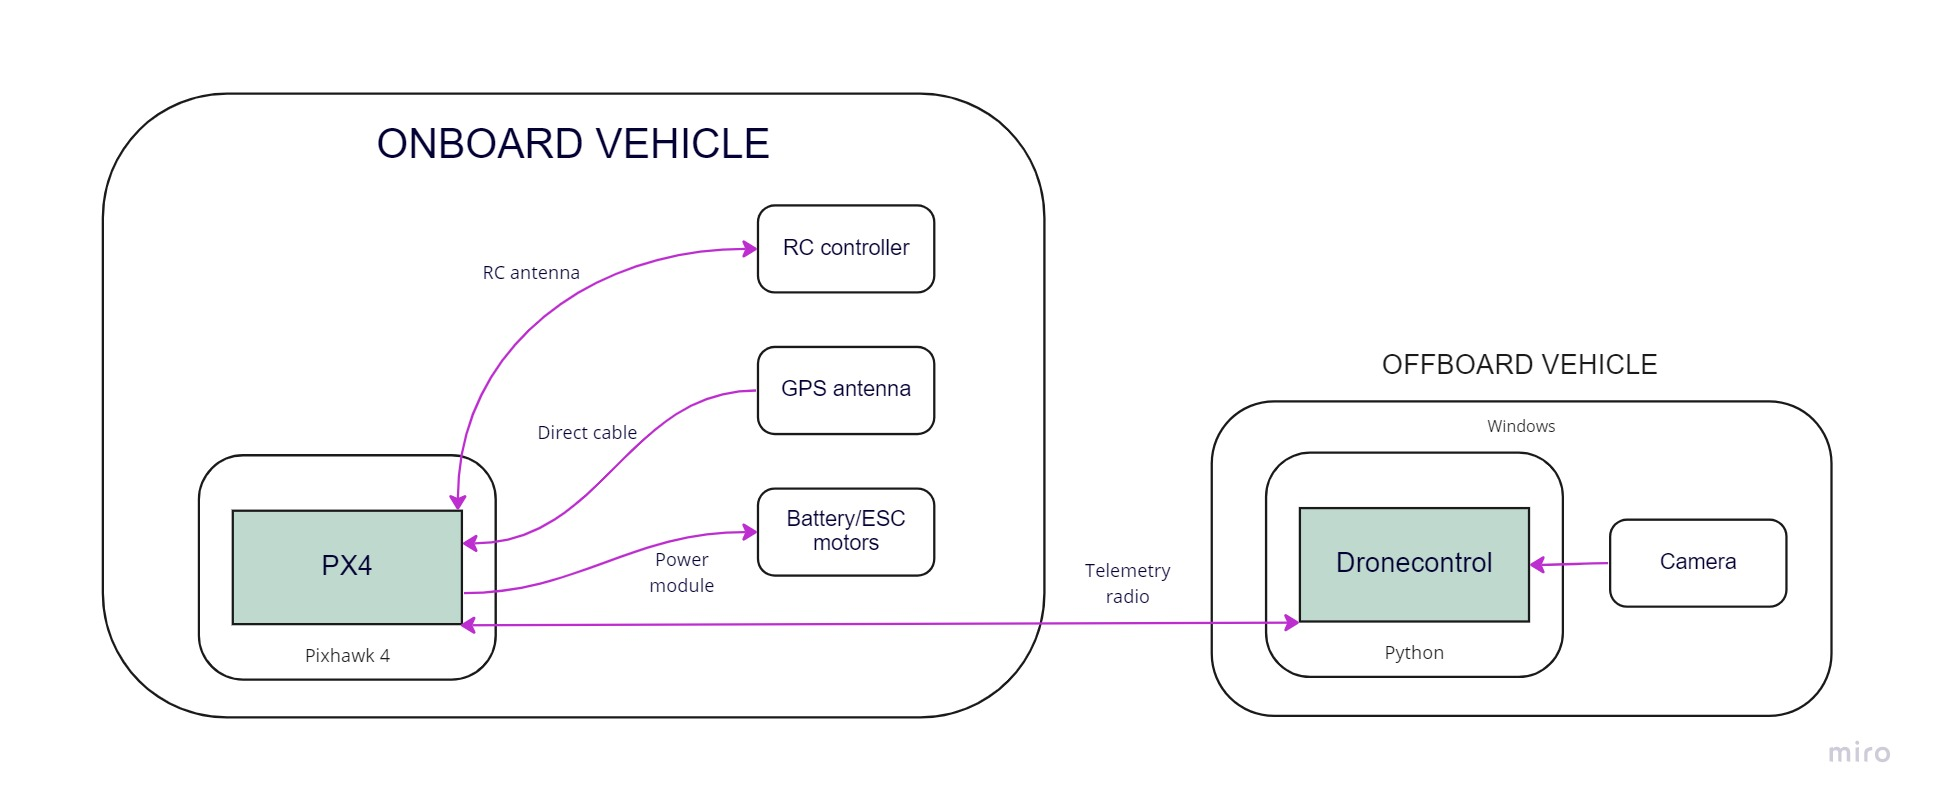
\includegraphics[width=\textwidth,keepaspectratio]{img/offboard-diagram.jpg}
  \caption{Offboard configuration connections.}
  \label{fig:offboard-config}
\end{figure}

The offboard configuration allows the flight controller to communicate and receive orders from a companion computer that is not physically connected to its hardware, so the latter can remain on the ground while the vehicle flies.
This configuration offers several advantages, including a simplified setup without concerns about hardware interactions and power supply to the companion computer during flight. It also allows for the use of a more powerful computer for image processing without adding weight to the vehicle. However, the camera remains connected to the ground computer, limiting the system's real-world applications as the images are not captured from the drone's perspective during flight. While other configurations involving direct camera-to-flight controller connection and wireless transmission of images for offboard processing are feasible, they are beyond the scope of this project. Figure \ref{fig:offboard-config} provides a summary of the connections required for the offboard computer configuration setup, including the PX4 software, the DroneVisionControl application, their respective hardware platforms, and onboard and ground station peripherals.

In this configuration, the wireless link is established through a pair of telemetry radios.
These radios connect to a telemetry port on the flight controller and a USB port on the companion computer. 
Since the Pixhawk 4 is configured by default to use its \texttt{TELEM1} port for this purpose, no additional configuration is needed when using that port.
Applications like the QGRoundControl ground station software automatically detect a telemetry radio inserted into any USB port on the host computer and establish the connection to the flight controller.
Additionally, software using the MAVSDK library can establish a connection by specifying the USB serial port address and the baudrate of the link, usually something similar to \texttt{/dev/ttyUSB0:57600} on Linux and \texttt{COM1:57600} on Windows.

The project utilizes the Holybro SiK Telemetry Radio\footnote{\url{http://www.holybro.com/product/transceiver-telemetry-radio-v3/}} for physical tests. These radios are small, lightweight, and cost-effective, offering a range of more than 300 meters (which can be extended with a patch antenna). They operate at either 915MHz (Europe) or 433MHz (US), complying with regional frequency regulations. The radios support two-way full-duplex communication through an adaptive TDM UART interface, with an adjustable maximum output power of 100mW and a receive sensitivity of -117dBm. The default baudrate for the connection is 57600, and the radios can achieve exchange rates of up to 250kbps.


\subsection{Onboard computer configuration}
\label{subsec:onboard}

The second way of configuring the interaction between the flight controller and the companion computer consists of incorporating both of them together on board the UAV.
This is achieved by connecting the flight controller directly to the companion computer using a serial cable.
The camera will also be onboard the vehicle, attached to the frame in a way that allows for a practical perspective during flight.
This configuration makes it possible to develop new control solutions based on images taken directly from the vehicle, creating a feedback loop that adjusts to maintain a stable output based on the reaction of the vehicle to commands.
Figure \ref{fig:onboard-config} shows a summary of all the connections present in the onboard configuration between the three pieces of software that interact together: PX4, DroneVisionControl and QGroundControl, with their respective hardware platforms and the attached peripherals.

\begin{figure}[b!]
  \centering
  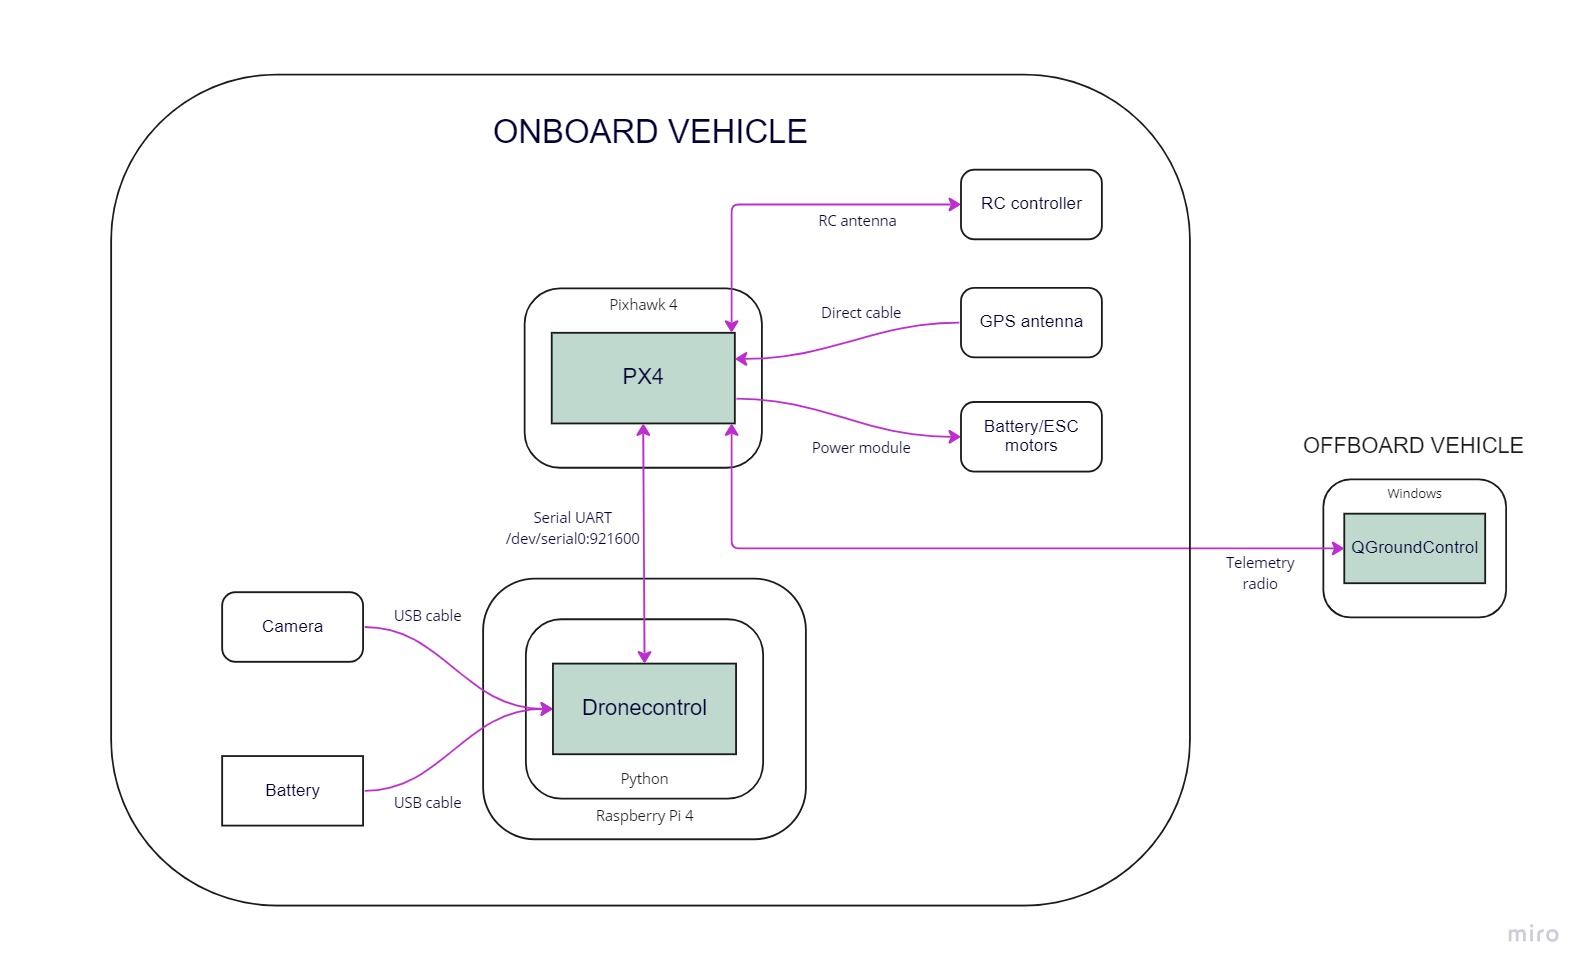
\includegraphics[width=0.85\textwidth,keepaspectratio]{img/onboard-diagram.jpg}
  \caption{Overview of the onboard configuration. All connections are contained inside the vehicle's frame.}
  \label{fig:onboard-config}
\end{figure}


Selecting the appropriate hardware for the onboard computer is crucial in this configuration since the companion computer has to fly along with the flight controller. 
To be able to take into the air, the computer has to be light enough that its weight can be lifted by the propellers while maintaining adequate battery autonomy.
It also needs to be powerful enough that its processor can handle computer vision algorithms.
The Raspberry Pi 4 model chosen for this project and shown in Figure \ref{fig:rpi4-pinout} is one of the most popular small computers available in the market at the time, and it is widely used in all kinds of robotics projects both for education and hobbyists. 
One of the most crucial advantages of using such a platform is the excellent availability of manuals, guides, and other support found on the web. 
In addition, the Raspberry’s officially supported operating
system, called Raspberry Pi OS, is a Debian-based version of Unix, which simplifies the transition from the WSL test environment.

\begin{figure}[H]
  \centering
  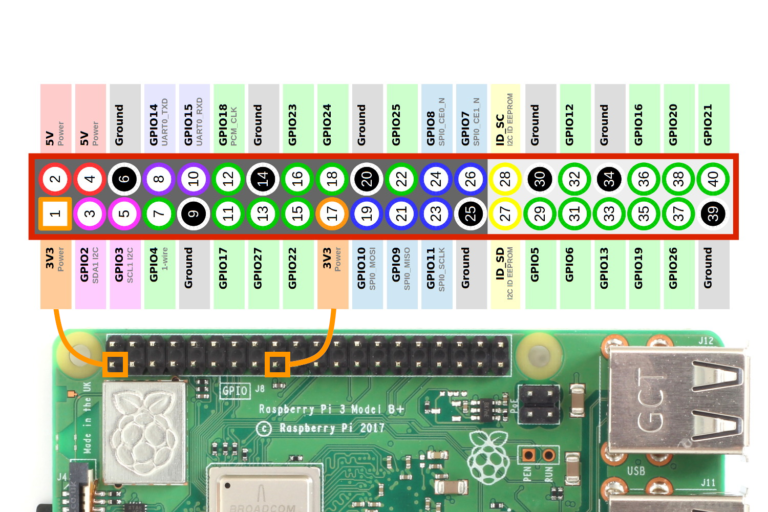
\includegraphics[width=0.8\textwidth,keepaspectratio]{img/rpi4-pinout.png}
  \caption{The Raspberry Pi microcomputer, with its 40-pin GPIO header marked in red and annotated pinout.}
  \source{Adapted from \citetitle{rpi4-pinout} \cite{rpi4-pinout}}
  \label{fig:rpi4-pinout}
\end{figure}

Since this computer is designed for integration with hardware projects, it includes a 40-pin \acrfull{gpio} header (highlighted in Figure \ref{fig:rpi4-pinout}) for connecting external devices.
This pin header, along with the standard ports in the Raspberry Pi, will be used to implement the three connections to the companion computer required for the onboard configuration, shown in Figure \ref{fig:wiring}.
The first connection will provide power to the computer, the second will be a connection to the camera that provides images, and the third one will be the telemetry link to the flight controller.

\begin{figure}
  \centering
  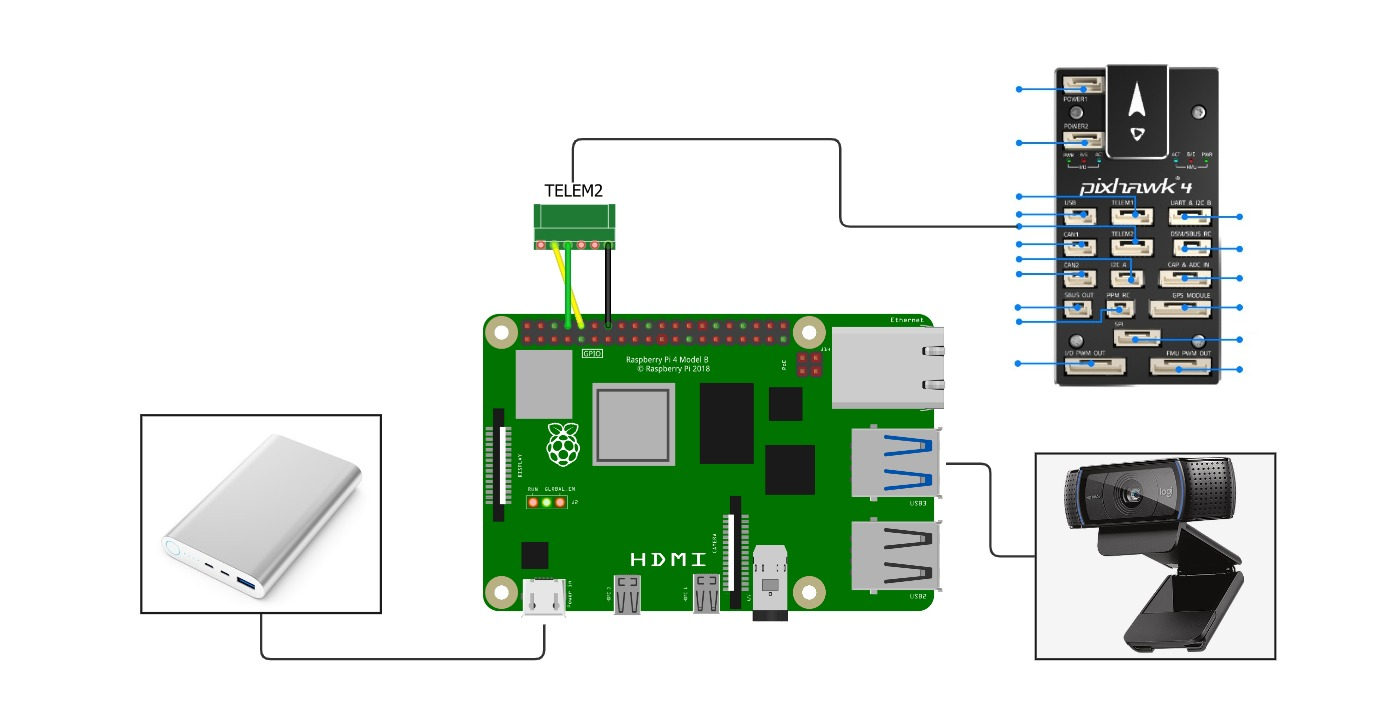
\includegraphics[width=\textwidth,keepaspectratio]{img/wiring-diagram.jpg}
  \caption{A diagram of the wired connections from the Raspberry Pi 4 to the secondary battery and the flight controller (\texttt{TELEM2}).}
  \label{fig:wiring}
\end{figure}

The Raspberry Pi is powered by a 5V input that can be supplied via the USB-C port or specific pins on the GPIO header ("5v Power" on Figure \ref{fig:rpi4-pinout}). 
In the specific vehicle build of this project, the Holybro PM07\footnote{\url{http://www.holybro.com/product/pixhawk-4-power-module-pm07/}} power management board supplies 5V to the flight controller and powers the ESCs for the motors. 
The power management board features two power outputs: one connected to the flight controller's \texttt{POWER1} port and an unused one. 
Initially, attempts were made to power the Raspberry Pi from the main battery by connecting the second output on the power module to the GPIO header's powering pins using a custom connector. 
However, this resulted in an unstable power supply for the Pi board, causing frequent current dips that affected the companion computer's processing capabilities. 
To address this, a secondary battery was introduced, providing power to the Raspberry Pi via a USB to USB-C cable. 
This configuration allows the Raspberry Pi to receive power through its default regulated USB-C port. 
The drawback is the additional weight of the secondary battery, which also needs to be securely attached to the vehicle's frame during flight.

In contrast to selecting a companion computer, the choice of camera for the onboard system offers greater flexibility. The key considerations are lightweight design and straightforward plug-and-play compatibility with the onboard computer. The camera utilized in the tests outlined in Chapter \ref{chap:validation} is the Logitech C920 1080p webcam\footnote{\url{https://www.logitech.com/es-es/products/webcams/c920-pro-hd-webcam.960-001055.html}} described in Section \ref{subsec:camera}. Since the Holybro X500 frame doesn't natively support an onboard camera, a custom mount was designed and 3D-printed using PLA plastic. This mount securely attaches the camera to the underside of the vehicle frame's central rods, ensuring stability during flight. The 3D model of the mount is depicted in Figure \ref{fig:camera-holder-3d}, and the print-ready file is available in the project's repository in GitHub\footnote{\url{https://github.com/l-gonz/tfg-giaa-dronecontrol/blob/main/data/camera-holder.stl}}.

\begin{figure}
  \centering
  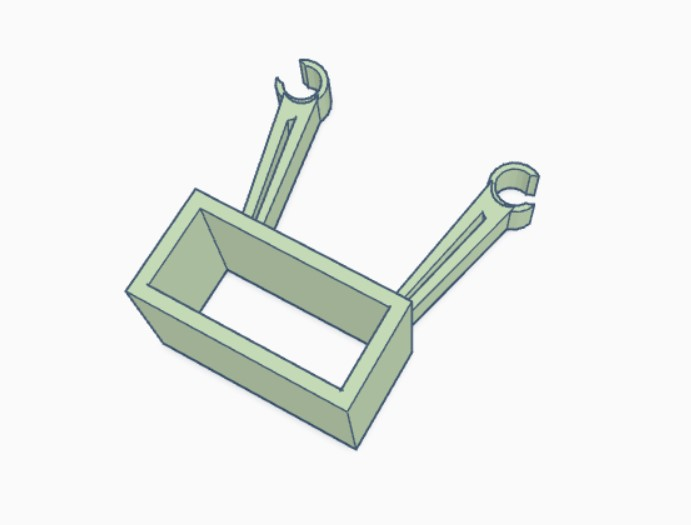
\includegraphics[width=0.6\textwidth, keepaspectratio]{img/cam-holder.jpg}
  \caption{3D model for the camera mount designed for the Holybro X500 frame.}
  \label{fig:camera-holder-3d}
\end{figure}

The last wired connection that needs to be established for this configuration is between the flight controller and the companion computer for MAVLink message exchange.
This connection will use the secondary telemetry port of the flight controller, \texttt{TELEM2}.
Meanwhile, the telemetry radio will remain connected to the \texttt{TELEM1} port to maintain a wireless link.
This link can be employed by a ground station (QGroundControl) to override the companion computer's control during flight.
The telemetry connections on the flight controller use a 6-pin adapter to attach to the \texttt{TELEM} ports.
On the Raspberry Pi side, the other end of the connector has three female Dupont wires that connect to the TX/RX UART pins. The pins in the telemetry port are mapped to the corresponding GPIO pins on the Raspberry Pi's header according to the wiring provided in Table \ref{tab:wiring-telem}. This wiring configuration is also depicted in the diagram in Figure \ref{fig:wiring}.

\begin{table}[ht]
\centering
\begin{tabular}{|ll||ll|}
\hline
\multicolumn{2}{|c||}{\textbf{TELEM2}}                                             & \multicolumn{2}{c|}{\textbf{GPIO header}}                                        \\ \hline \hline
\multicolumn{1}{|c|}{\textit{Pin \#}} & \multicolumn{1}{c||}{\textit{Description}} & \multicolumn{1}{c|}{\textit{Description}} & \multicolumn{1}{c|}{\textit{Pin \#}} \\ \hline
\multicolumn{1}{|l|}{1}               & VCC, +5V                                  & \multicolumn{1}{l|}{}                     &                                      \\ \hline
\multicolumn{1}{|l|}{2}               & TX (out), +3.3V                           & \multicolumn{1}{l|}{GPIO15 (RXD0, UART)}  & 10                                   \\ \hline
\multicolumn{1}{|l|}{3}               & RX (in), +3.3V                            & \multicolumn{1}{l|}{GPIO14 (TXD0, UART)}  & 8                                    \\ \hline
\multicolumn{1}{|l|}{4}               & CTS (in), +3.3V                           & \multicolumn{1}{l|}{}                     &                                      \\ \hline
\multicolumn{1}{|l|}{5}               & RTS (in), +3.3V                           & \multicolumn{1}{l|}{}                     &                                      \\ \hline
\multicolumn{1}{|l|}{6}               & GND                                       & \multicolumn{1}{l|}{GND}                  & 6                                    \\ \hline
\end{tabular}
\caption{Mapping between the \texttt{TELEM2} port in the Pixhawk 4 board and the Raspberry Pi's GPIO header.}
\label{tab:wiring-telem}
\end{table}

By default, the secondary telemetry port, \texttt{TELEM2}, is not enabled for use.
Its configuration can be changed through a ground station computer connected to the Pixhawk board by using the Parameters section of the QGroundControl application.
The specific parameters that need to be set are discussed in Section \ref{sec:test-5-rpi}.


Compared to the default baud rate of 57600 used for the telemetry radio link established earlier, the wired serial connection operates at a faster rate of 921600. This means that data can be transferred up to 16 times faster through this link. However, it is important to note that the primary limitation on speed for the program lies in the detection and tracking process running on the images. Therefore, a faster link rate does not necessarily result in an overall performance improvement for the solution. In Section  \ref{subsec:performance}, different hardware combinations are analyzed to identify any challenges that may impact the program's performance.

Moving beyond the individual hardware components, it is important to compare the use of this onboard configuration with the previously discussed offboard configuration during testing. While the offboard setup allowed for monitoring the program's output by connecting a screen directly to the companion computer on the ground, such a setup is not feasible in the onboard configuration. However, a solution to this limitation is to leverage the Raspberry Pi's WiFi antenna and configure a remote desktop connection. By connecting to this remote desktop from another computer acting as a ground station, real-time monitoring of the camera output and image recognition can be achieved, along with the capability to provide direct input during flight.